\section{Introduction}
Depth estimation is one of the most researched areas in computer vision.
While traditionally sparse stereo correspondence algorithms were used, most modern work is concerned with estimating dense depth maps from images.
Typically, this is achieved via a stereo matching approach, in which (under certain assumptions about epipolar geometry and the appearance of surfaces) a disparity map can be computed by warping one image of a stereo  pair into the other.
As described by Scharstein \& Szeliski~\cite{scharstein2002taxonomy}, this usually involves an appearance cost function, a global smoothness constraint and iterative refinements of depth maps.
Most contemporary approaches still make use of these basic ingredients.

Stereo-based approaches have the inherent disadvantages that they require a stereo image pair for each newly generated depth estimate.
The respective stereo data, however, is not available for the majority of use-cases.
This has sparked research into monocular depth estimation methods, which are usually based on machine learning models trained on large amounts of ground truth depth data.
Ground truth depth data, however, is very tedious to capture. 
It requires the use of expensive and finely calibrated depth scanning hardware such as LiDAR sensors. These introduce further problems including noise in distant samples, sparse measuring, as well as sensor calibration difficulties. Therefore, ground truth depth data is not available in large quantities for most scenarios.
The KITTI Stereo dataset from 2015 for example\cite{Menze2015CVPR}, consisting of only 200 images, was captured using a LiDAR sensor and consequently, depth is only available for about 5\% of the pixels and only for non-moving objects. 

Because of this, recent monocular depth estimation methods~\cite{garg2016unsupervised,Godard_2017_CVPR,Godard2018} approach the estimation process as an unsupervised image reconstruction problem, in which stereo or video data is only required during training and can easily be captured with modern smartphones, for example. 
The monocular depth estimation architecture by Godard \etal~\cite{Godard_2017_CVPR} demonstrated that when enforcing consistency between two predicted depth maps and the two camera views, superior performance to fully-supervised baselines and generalization to yet unseen datasets can be achieved.
Most of their depth estimates' uncertainty can be found in uniform regions and at object boundaries. 

This is not surprising, since dense predictions tasks, such as semantic segmentation and depth estimation, face two key challenges: Capturing rich contextual information and detecting objects at multiple scales, while also maintaining sharp object boundaries in the final dense prediction.
State of the art CNN architectures typically use small filter sizes, repeated striding operations and max-pooling to down-sample the image, which reduce the resolution of feature maps and as a result make details difficult to recover.
As mentioned by Fu \etal~\cite{Fu2018}, previous solutions include the use of skip-connections~\cite{Ronneberger2015}, iterative refinement or multi-layer deconvolution networks~\cite{noh2015learning}. 
\begin{figure}
    \centering
    \begin{subfigure}[b]{0.35\linewidth}
    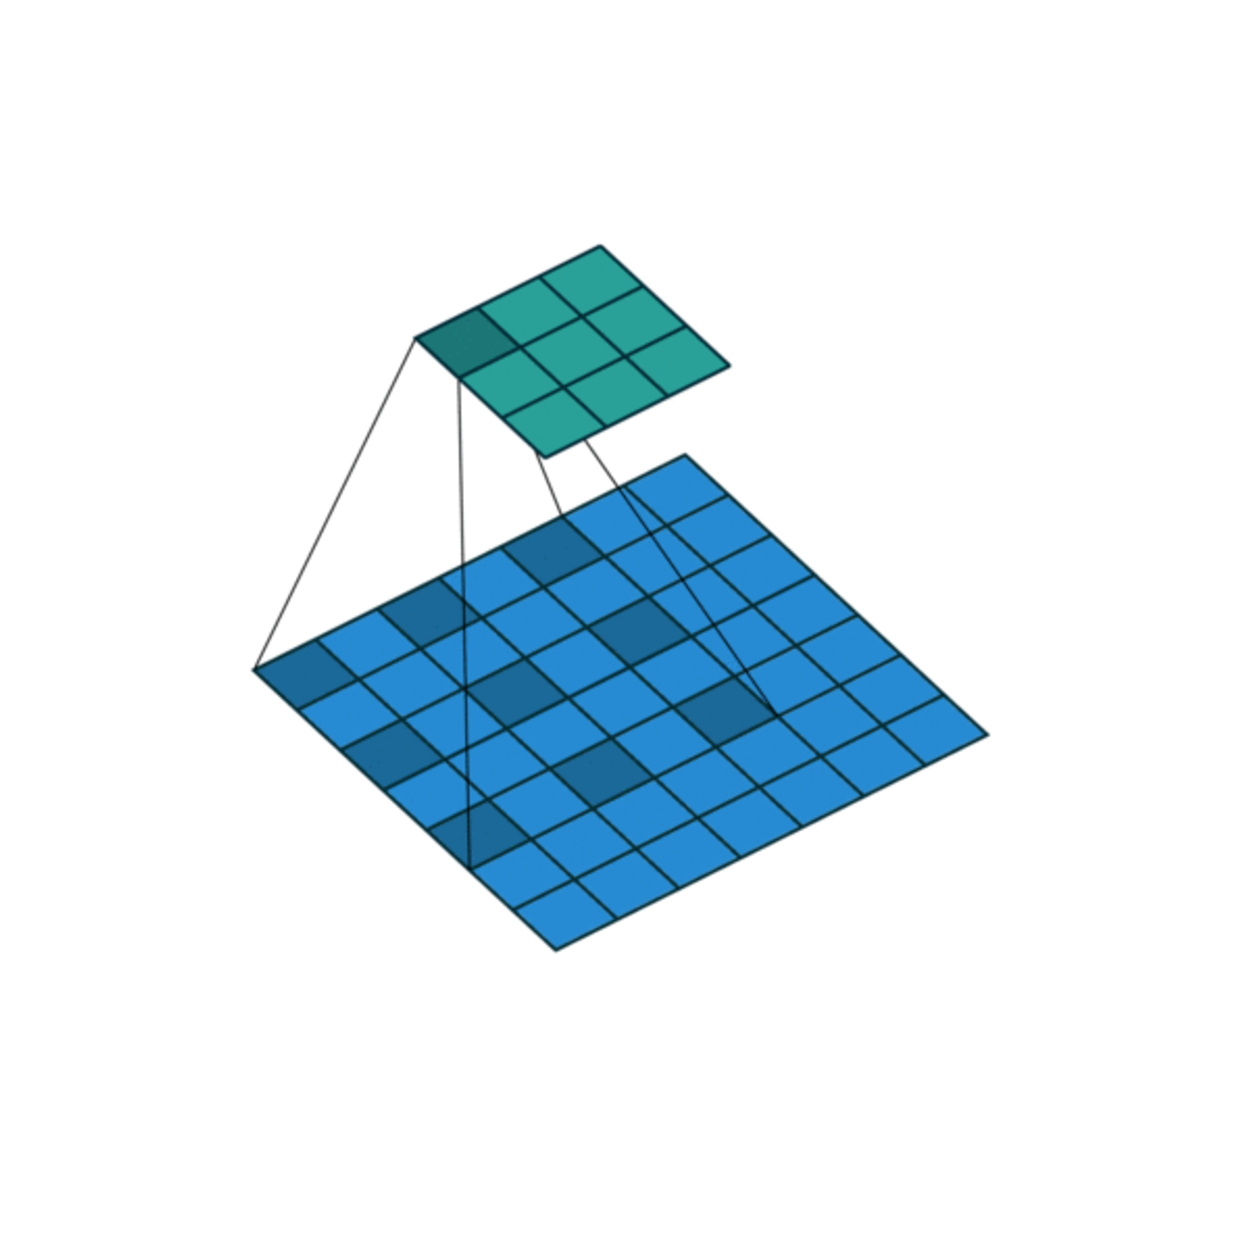
\includegraphics[width=1.0\linewidth]{images/concepts/dilation.pdf}
    \caption{}
    \label{fig:atrous-convolution}
    \end{subfigure}
    \begin{subfigure}[b]{0.6\linewidth}
        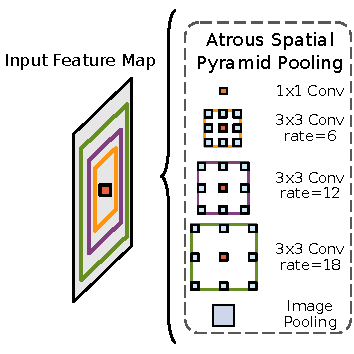
\includegraphics[width=1.0\linewidth]{images/architecture/aspp.pdf}
        \caption{}
        \label{fig:aspp}
    \end{subfigure}
    \caption{(a) Atrous convolution with a dilation rate of 2. (b) Atrous Spatial Pyramid Pooling (ASPP). The field of views of the different atrous convolutions are shown in different colors on the input feature map. Figure adapted from Chen \etal~\cite{chen2018deeplab}.}
\end{figure}

In this work, we investigate whether atrous convolutions, which have proven successful in semantic segmentation~\cite{chen2018deeplab, chen2018encoder}, can also improve monocular depth estimation.
Atrous convolutions allow to explicitly control the receptive field size of a filter without introducing additional parameters.
This is achieved by skipping pixels at a certain rate (also called filter dilation), and thus inserting zero holes (french: \textit{trous}) into the filter (see \figurename~\ref{fig:atrous-convolution}).
This helps with aggregating information from different spatial scales, while also allowing for larger feature maps, as less downsampling is required in order to achieve a large field of view (FOV). 

With these considerations in mind, we designed an architecture using atrous convolutions based on the original monocular depth estimation architecture from Godard \etal~\cite{Godard_2017_CVPR}, and we compare this both visually and quantitatively to the original baseline. In the architecture design, we considered predictive performance and runtime and memory consumption.
We performed several experiments that show how these factors are influenced by different architectural decisions.
We conclude that atrous convolutions, at least in the setups we investigated, do not improve monocular depth estimation. 
Based on our experiments we propose an architecture that improves upon the baseline performance from Gordard \etal~\cite{Godard_2017_CVPR} while cutting the number of parameters by 24.5\%. 

